\documentclass[11pt]{article}

% Change "review" to "final" to generate the final (sometimes called camera-ready) version.
% Change to "preprint" to generate a non-anonymous version with page numbers.
\usepackage[preprint]{acl}

% Standard package includes
\usepackage{times}
\usepackage{latexsym}
\usepackage{amsmath}
\usepackage{fvextra}
\usepackage{pgfplots}
\pgfplotsset{compat=1.18}
\usepgfplotslibrary{groupplots}
\usepackage{booktabs}
\usepackage{longtable}

\DefineVerbatimEnvironment{PromptVerbatim}{Verbatim}{
    fontsize=\scriptsize,
    breaklines=true,
    breaksymbolleft={},
}

\usepackage{xcolor}
\definecolor{creeblue}{RGB}{31,119,180}
\definecolor{enorange}{RGB}{255,127,14}
\definecolor{guaranigreen}{RGB}{0,158,115}
% cyan/purple-blue pair for BPE vs MorphBPE (Figures 2-4 below), adapted
% from the source paper's own figure palette -- see report/figures/
% fertility.tex for why the exact sampled hex values needed adjusting.
\definecolor{bpecolor}{HTML}{0D9BD0}
\definecolor{morphbpecolor}{HTML}{8B5FDB}

% For proper rendering and hyphenation of words containing Latin characters (including in bib files)
\usepackage[T1]{fontenc}
% For Vietnamese characters
% \usepackage[T5]{fontenc}
% See https://www.latex-project.org/help/documentation/encguide.pdf for other character sets

% This assumes your files are encoded as UTF8
\usepackage[utf8]{inputenc}

% This is not strictly necessary, and may be commented out,
% but it will improve the layout of the manuscript,
% and will typically save some space.
\usepackage{microtype}

% This is also not strictly necessary, and may be commented out.
% However, it will improve the aesthetics of text in
% the typewriter font.
\usepackage{inconsolata}

%Including images in your LaTeX document requires adding
%additional package(s)
\usepackage{graphicx}

\usepackage[most]{tcolorbox}

\tcbset{
    promptbox/.style={
        colback=gray!5,
        colframe=gray!60,
        boxrule=0.4pt,
        arc=1mm,
        left=2mm,
        right=2mm,
        top=1mm,
        bottom=1mm,
        enhanced
    }
}

% If the title and author information does not fit in the area allocated, uncomment the following
%
%\setlength\titlebox{<dim>}
%
% and set <dim> to something 5cm or larger.

\title{MorphBPE for Low-Resource Polysynthetic Languages}

\author{Konrad Brüggemann \\
  University of Tübingen\\
  \texttt{konrad-rudolf.brueggemann@student.uni-tuebingen.de}}

\begin{document}
\maketitle

\begin{abstract}
MorphBPE is a morphologically informed variant of the BPE algorithm for tokenization, which uses a morpheme lexicon during training. We propose a method to expand MorphBPE to languages for which no manually morpheme-segmented data exist. Essentially, we employ unsupervised methods to produce the segmentations, or, if available, morphological analyzers such as finite-state transducers. While MorphBPE is most effective with high quality morpheme-segmented data, we show that our approach still outperforms standard BPE in low-resource polysynthetic language settings.
\end{abstract}

\section{Introduction}

\section{Related Work}

\section{Data}

Table~\ref{tab:token-stats} reports the size and average morphological complexity of the training-split boundary lexicons used for all three languages, computed from Morfessor segmentations backed by a rule-based analyzer (\texttt{lang-crk} for Cree, Uqailaut for Inuktitut, \texttt{apertium-grn} for Guarani) where one is available.

\begin{table*}[t]
\centering
\begin{tabular}{llrr}
\toprule
Language & Morphology Type & \# Word Types & Avg. Morphemes/Word \\
\midrule
Cree      & Polysynthetic (preverb + stem + suffixes)          & 17{,}707  & 2.47 \\
Inuktitut & Polysynthetic (root + productive suffix chains)    & 423{,}450 & 2.50 \\
Guarani   & Agglutinative (verb agreement + noun incorporation) & 46{,}754  & 1.84 \\
\bottomrule
\end{tabular}
\caption{Token statistics for the morphological boundary lexicons used in BPE and \textit{MorphBPE} training and tokenizer evaluation.}
\label{tab:token-stats}
\end{table*}

\section{Methods}

\section{Experimental Setup}

\section{Results}

Table~\ref{tab:consistency} reports Consistency F1, precision, and recall for both tokenizers across all three languages, showing that \textit{MorphBPE} achieves substantially higher morphological consistency than standard BPE in every case.

\begin{table*}[t]
\centering
\begin{tabular}{lccc}
\toprule
Model & Precision & Recall & Morph.-Consistency F1-score \\
\midrule
Cree BPE (1K)                    & 0.22 & 0.33 & 0.27 \\
Cree \textit{MorphBPE} (1K)      & 0.36 & 0.69 & \textbf{0.47} \\
\addlinespace
Inuktitut BPE (8K)               & 0.44 & 0.21 & 0.28 \\
Inuktitut \textit{MorphBPE} (8K) & 0.62 & 0.50 & \textbf{0.56} \\
\addlinespace
Guarani BPE (3K)                 & 0.07 & 0.28 & 0.11 \\
Guarani \textit{MorphBPE} (3K)   & 0.14 & 0.66 & \textbf{0.24} \\
\bottomrule
\end{tabular}
\caption{Morph.-consistency evaluation: Precision, Recall, and F1-score for BPE and \textit{MorphBPE}, Plains Cree, Inuktitut, and Guarani. Single evaluation run on the held-out test split (no resampling); a higher F1-score indicates greater consistency in segmenting words with similar or dissimilar morphemes.}
\label{tab:consistency}
\end{table*}

Figures~\ref{fig:fertility} and \ref{fig:morph-edit-distance} compare Fertility and Morph Edit Distance for both tokenizers across all three languages (Consistency F1 is already broken down by Precision/Recall in Table~\ref{tab:consistency} above, so it isn't re-plotted here), showing that \textit{MorphBPE}'s higher fertility is consistently offset by a lower Morph Edit Distance, though the effect is more muted for Guarani (see the Limitations section).

\begin{figure}[t]
\centering
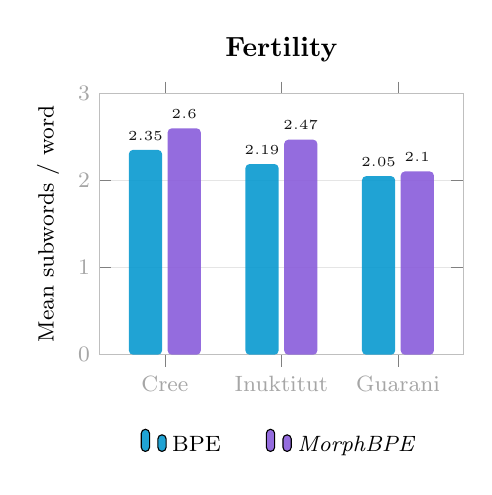
\begin{tikzpicture}
\begin{axis}[
    width=6.2cm, height=4.9cm,
    title={Fertility},
    title style={color=black, font=\bfseries\normalsize, yshift=2pt},
    ybar,
    bar width=12pt,
    enlarge x limits=0.28,
    symbolic x coords={Cree,Inuktitut,Guarani},
    xtick=data,
    ymin=0, ymax=3.0,
    ylabel={Mean subwords / word},
    tick label style={color=gray!70, font=\footnotesize},
    label style={color=black, font=\footnotesize},
    axis line style={gray!50},
    ymajorgrids=true,
    xmajorgrids=false,
    grid style={gray!20, line width=0.5pt},
    every axis plot/.append style={draw=none, fill opacity=0.92, rounded corners=1.5pt},
    nodes near coords style={font=\tiny, color=black},
    nodes near coords, every node near coord/.append style={/pgf/number format/.cd, fixed, precision=2},
    legend style={
        at={(0.5,-0.26)}, anchor=north,
        legend columns=-1,
        font=\footnotesize, draw=none, fill=none,
        /tikz/every even column/.append style={column sep=0.5cm},
    },
    legend cell align=left,
]
\addplot[fill=bpecolor] coordinates {(Cree,2.351932428973637) (Inuktitut,2.189355277064774) (Guarani,2.050191264870318)};
\addlegendentry{BPE}
\addplot[fill=morphbpecolor] coordinates {(Cree,2.599180957256207) (Inuktitut,2.468730182696663) (Guarani,2.104207827147001)};
\addlegendentry{\textit{MorphBPE}}
\end{axis}
\end{tikzpicture}
\caption{Fertility for BPE vs.\ \textit{MorphBPE}, Plains Cree, Inuktitut, and Guarani.}
\label{fig:fertility}
\end{figure}

\begin{figure}[t]
\centering
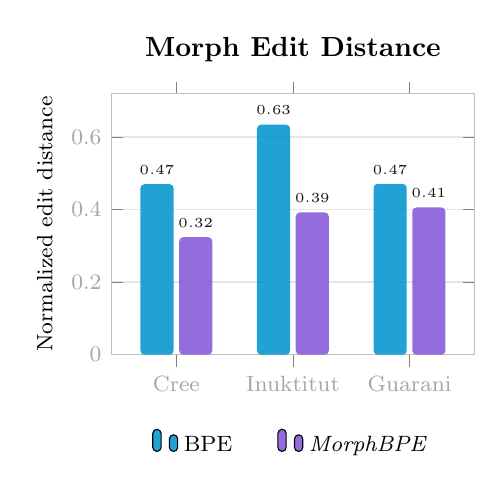
\begin{tikzpicture}
\begin{axis}[
    width=6.2cm, height=4.9cm,
    title={Morph Edit Distance},
    title style={color=black, font=\bfseries\normalsize, yshift=2pt},
    ybar,
    bar width=12pt,
    enlarge x limits=0.28,
    symbolic x coords={Cree,Inuktitut,Guarani},
    xtick=data,
    ymin=0, ymax=0.72,
    ylabel={Normalized edit distance},
    tick label style={color=gray!70, font=\footnotesize},
    label style={color=black, font=\footnotesize},
    axis line style={gray!50},
    ymajorgrids=true,
    xmajorgrids=false,
    grid style={gray!20, line width=0.5pt},
    every axis plot/.append style={draw=none, fill opacity=0.92, rounded corners=1.5pt},
    nodes near coords style={font=\tiny, color=black},
    nodes near coords, every node near coord/.append style={/pgf/number format/.cd, fixed, precision=2},
    legend style={
        at={(0.5,-0.26)}, anchor=north,
        legend columns=-1,
        font=\footnotesize, draw=none, fill=none,
        /tikz/every even column/.append style={column sep=0.5cm},
    },
    legend cell align=left,
]
\addplot[fill=bpecolor] coordinates {(Cree,0.47010415887966944) (Inuktitut,0.6340606341184748) (Guarani,0.47096764279078007)};
\addlegendentry{BPE}
\addplot[fill=morphbpecolor] coordinates {(Cree,0.3237583165134182) (Inuktitut,0.39202809066292077) (Guarani,0.4058784538693111)};
\addlegendentry{\textit{MorphBPE}}
\end{axis}
\end{tikzpicture}
\caption{Morph Edit Distance for BPE vs.\ \textit{MorphBPE}, Plains Cree, Inuktitut, and Guarani.}
\label{fig:morph-edit-distance}
\end{figure}

Figure~\ref{fig:training-loss} shows that the small diagnostic language models trained on \textit{MorphBPE}-tokenized text converge to a lower cross-entropy loss than those trained on standard BPE, for all three languages. Unlike the source paper, our two model sizes don't share the same language set -- Cree and Guarani only exist at the smaller ($\sim$1.3M-parameter) scale, Inuktitut only at the larger ($\sim$3.1M-parameter) one (see the Limitations section) -- so panel (a) and panel (b) below are split by model size rather than both showing all languages, and only the within-language BPE-vs-\textit{MorphBPE} direction should be read across panels, not the curves' absolute scale.

\begin{figure*}[t]
\centering
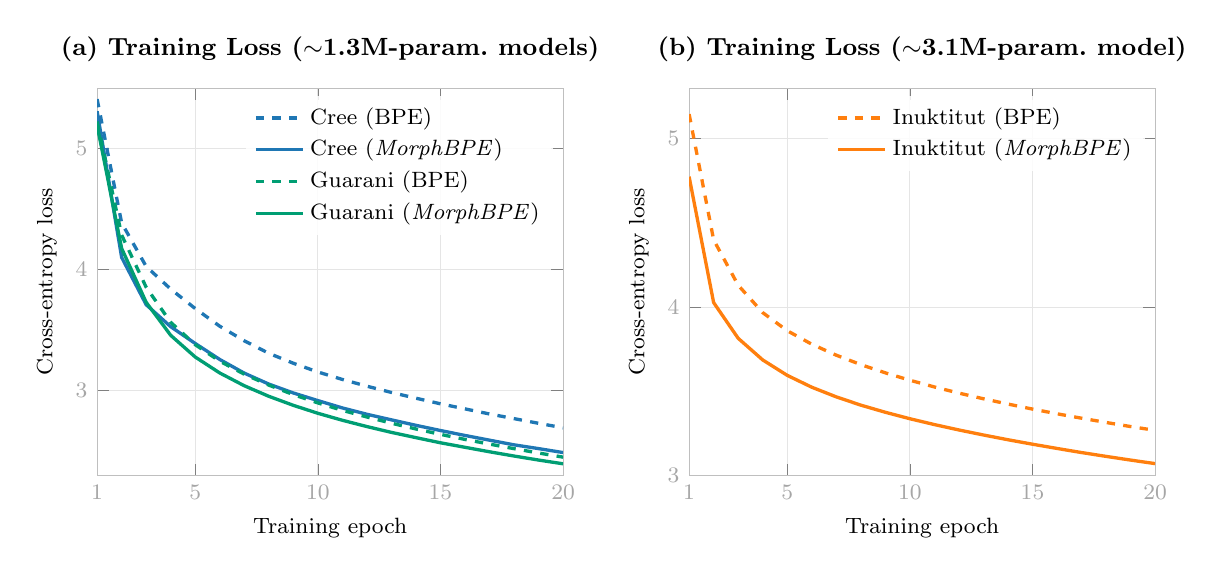
\begin{tikzpicture}
\begin{groupplot}[
    group style={
        group size=2 by 1,
        horizontal sep=1.6cm,
    },
    width=7.5cm, height=6.5cm,
    xlabel={Training epoch},
    ylabel={Cross-entropy loss},
    xmin=1, xmax=20,
    xtick={1,5,10,15,20},
    grid=major,
    grid style={gray!20, line width=0.3pt},
    axis line style={gray!50},
    tick label style={color=gray!70, font=\footnotesize},
    label style={color=black, font=\footnotesize},
    title style={color=black, font=\bfseries\small},
    legend style={
        font=\footnotesize,
        draw=none,
        fill=white,
        fill opacity=0.85,
        text opacity=1,
        at={(0.98,0.98)},
        anchor=north east,
    },
    legend cell align=left,
    every axis plot/.append style={line width=1.2pt, mark=none},
]

\nextgroupplot[title={(a) Training Loss ($\sim$1.3M-param.\ models)}, ymin=2.3, ymax=5.5]
\addplot[creeblue, dashed] coordinates {
    (1,5.409744389851888) (2,4.386526346206665) (3,4.026913932959238)
    (4,3.839942232767741) (5,3.679182934761047) (6,3.533221205075582)
    (7,3.4127057075500487) (8,3.3093050122261047) (9,3.227153480052948)
    (10,3.155119327704112) (11,3.093248935540517) (12,3.0376282731691995)
    (13,2.985764479637146) (14,2.9383687456448873) (15,2.8919909795125327)
    (16,2.85012233654658) (17,2.8080217401186625) (18,2.7696027636528013)
    (19,2.730829155445099) (20,2.6938249349594114)
};
\addlegendentry{Cree (BPE)}

\addplot[creeblue, solid] coordinates {
    (1,5.309244427314171) (2,4.10192165007958) (3,3.7109610374157245)
    (4,3.529307277386005) (5,3.390667618238009) (6,3.258465106670673)
    (7,3.1455732895777775) (8,3.05503328029926) (9,2.981681966781616)
    (10,2.9186128579653228) (11,2.857948974462656) (12,2.8056417281811052)
    (13,2.7595270230219913) (14,2.7142072897690994) (15,2.67128178523137)
    (16,2.630489947245671) (17,2.5915081427647517) (18,2.5529855508070725)
    (19,2.5217796949239877) (20,2.4891653501070463)
};
\addlegendentry{Cree (\textit{MorphBPE})}

\addplot[guaranigreen, dashed] coordinates {
    (1,5.224725457659939) (2,4.286658115554274) (3,3.8551399467284218)
    (4,3.5652930987508675) (5,3.3806605328593338) (6,3.2443483335930003)
    (7,3.1365973395213746) (8,3.046502269150918) (9,2.9679102029716757)
    (10,2.899291479796694) (11,2.8378573812936483) (12,2.7830903603319537)
    (13,2.7316647872590183) (14,2.6840884298609016) (15,2.639471821617662)
    (16,2.597696984023379) (17,2.5590318702814874) (18,2.521374328094616)
    (19,2.4855177203814187) (20,2.451333114975377)
};
\addlegendentry{Guarani (BPE)}

\addplot[guaranigreen, solid] coordinates {
    (1,5.19164489877635) (2,4.176312266752638) (3,3.730721972111998)
    (4,3.458076004324288) (5,3.278673775237182) (6,3.1468275590189574)
    (7,3.0413718501041673) (8,2.954082681187268) (9,2.87938434810474)
    (10,2.8138099651912163) (11,2.75597928515796) (12,2.703983799136918)
    (13,2.655852682631591) (14,2.612422853708267) (15,2.5699227945557954)
    (16,2.5326147233617715) (17,2.4955053041721214) (18,2.460487581532577)
    (19,2.4272499156409295) (20,2.3962494926205995)
};
\addlegendentry{Guarani (\textit{MorphBPE})}

\nextgroupplot[title={(b) Training Loss ($\sim$3.1M-param.\ model)}, ymin=3.0, ymax=5.3]
\addplot[enorange, dashed] coordinates {
    (1,5.145976681575597) (2,4.398943669823224) (3,4.129752070980528)
    (4,3.967109422941198) (5,3.85960052912109) (6,3.7795338192461436)
    (7,3.7142577413953104) (8,3.6583696104903334) (9,3.6094431020512885)
    (10,3.565575699939906) (11,3.52565293297218) (12,3.4890820764678288)
    (13,3.4554464557089166) (14,3.4240319392143874) (15,3.3942550241266334)
    (16,3.3662945023454487) (17,3.340064173794486) (18,3.31474922701082)
    (19,3.2904876078153076) (20,3.2679009598487387)
};
\addlegendentry{Inuktitut (BPE)}

\addplot[enorange, solid] coordinates {
    (1,4.774372222896734) (2,4.026608575453351) (3,3.8146111439424186)
    (4,3.6861443357293924) (5,3.5945940554884914) (6,3.524129667309535)
    (7,3.466764019411111) (8,3.4176540975945566) (9,3.375257618932459)
    (10,3.3369444989289443) (11,3.302196471825999) (12,3.270154822935651)
    (13,3.2403360972125603) (14,3.2121411873990255) (15,3.18564347247035)
    (16,3.160443723601783) (17,3.1360984253174737) (18,3.1132796379886676)
    (19,3.0913377601371175) (20,3.0703356252306375)
};
\addlegendentry{Inuktitut (\textit{MorphBPE})}

\end{groupplot}
\end{tikzpicture}
\caption{Training cross-entropy loss over twenty epochs, BPE vs.\ \textit{MorphBPE}, split by LM model size: (a) Cree and Guarani ($\sim$1.3M-parameter models), (b) Inuktitut ($\sim$3.1M-parameter model).}
\label{fig:training-loss}
\end{figure*}

\section{Ablation}


\section{Discussion}

\section{Conclusion}
\label{sec:conclusion}

\section*{Limitations}

\section*{Ethical Considerations}

\bibliography{custom}
\appendix


\end{document}
